\section{光滑项与非光滑项的复合}
\label{sec:opt-ns-composite}

章首的$\ell_1$正则最小二乘有一个共同的结构：目标是一个光滑项与一个非光滑项之和，光滑项的梯度容易计算，非光滑项的邻近映射容易计算。本节研究这样的\term{复合目标}（composite objective）
\begin{equation}
 F(\bm x)=f(\bm x)+r(\bm x),
 \label{eq:opt-ns-composite}
\end{equation}
其中$f:\mathbb R^d\to\mathbb R$可微且梯度$L$-Lipschitz（第~\ref{chap:opt-smooth}章称为$L$光滑），$r$是适当、下半连续的凸函数，其邻近映射容易计算。对整个$F$用次梯度法，浪费了$f$的光滑性和$r$的简单结构；对整个$F$用邻近点法，子问题又太难。折中的办法是只近似$f$、完整保留$r$，并要求这样做仍能控制原目标$F$的进展。

\subsection{邻近梯度法}
\label{sec:opt-ns-proximal-gradient}

第~\ref{chap:opt-smooth}章的下降引理给出$L$光滑函数的二次上界：对所有$\bm x,\bm y$，
\begin{equation}
 f(\bm y)\leq f(\bm x)+\langle\nabla f(\bm x),\bm y-\bm x\rangle+\frac L2\lVert\bm y-\bm x\rVert_2^2 .
 \label{eq:opt-ns-descent-lemma}
\end{equation}
在那里，最小化右端得到梯度步$\bm x-\nabla f(\bm x)/L$。现在目标多了$r$。保留$r$不动，只把$f$换成它的二次上界，并把系数$L$换成$1/\eta$（$0<\eta\leq1/L$时这仍是上界），得到当前点$\bm x$处的模型
\[
 m_{\bm x}(\bm y)=f(\bm x)+\langle\nabla f(\bm x),\bm y-\bm x\rangle+\frac1{2\eta}\lVert\bm y-\bm x\rVert_2^2+r(\bm y).
\]

\paragraph{配方得到更新}
模型中关于$\bm y$的一次项和二次项可以配方：
\[
 \langle\nabla f(\bm x),\bm y-\bm x\rangle+\frac1{2\eta}\lVert\bm y-\bm x\rVert_2^2
 =\frac1{2\eta}\bigl\lVert\bm y-\bigl(\bm x-\eta\nabla f(\bm x)\bigr)\bigr\rVert_2^2-\frac\eta2\lVert\nabla f(\bm x)\rVert_2^2 .
\]
去掉与$\bm y$无关的项，最小化模型就是以梯度步的终点为中心求$r$的邻近映射。\term{邻近梯度法}（proximal gradient method）因此写成
\begin{equation}
 \bm x^{(t+1)}=\operatorname{prox}_{\eta r}\bigl(\bm x^{(t)}-\eta\nabla f(\bm x^{(t)})\bigr).
 \label{eq:opt-ns-proximal-gradient}
\end{equation}
一轮分两步：先对光滑项做一次显式梯度步，形成中心；再对非光滑项做一次隐式的邻近步。$r=0$时它退化为梯度下降；$f=0$时它就是邻近点法；$r=\iota_C$时邻近步是投影，得到第~\ref{chap:constrained-optimization}章的投影梯度法。

\begin{example}[二维Lasso的第一步]
\label{ex:opt-ns-lasso-step}
取$\bm A=\begin{pmatrix}1&1\\1&0\end{pmatrix}$、$\bm b=(1,2)^\top$、$\lambda=1$，目标$F(\bm x)=\frac12\lVert\bm A\bm x-\bm b\rVert_2^2+\lVert\bm x\rVert_1$。光滑部分的梯度为$\bm A^\top\bm A\bm x-\bm A^\top\bm b$，其中$\bm A^\top\bm A=\begin{pmatrix}2&1\\1&1\end{pmatrix}$、$\bm A^\top\bm b=(3,1)^\top$；最大特征值$L=(3+\sqrt5)/2\approx2.618$，取$\eta=1/4\leq1/L$。

从$\bm x^{(0)}=(-1,2)^\top$出发：梯度为$(-2+2-3,\ -1+2-1)^\top=(-3,0)^\top$，梯度步的中心是$(-1,2)^\top-\frac14(-3,0)^\top=(-0.25,2)^\top$；再以阈值$\eta\lambda=0.25$做软阈值，得$\bm x^{(1)}=(0,1.75)^\top$。第一个坐标被精确置零，目标值从$7.5$降到$4.03125$。

最优解可以由最优条件直接核验。猜测$x_2^\star=0$、$x_1^\star>0$：第一个坐标要求$2x_1-3+1=0$，得$x_1^\star=1$；第二个坐标要求$|[\bm A^\top(\bm b-\bm A\bm x^\star)]_2|=|1-x_1^\star|=0\leq1$，成立。所以$\bm x^\star=(1,0)^\top$，$F^\star=1.5$。只看光滑部分，最小点却是$(\bm A^\top\bm A)^{-1}\bm A^\top\bm b=(2,-1)^\top$。
\end{example}

图~\ref{fig:opt-ns-lasso-path}画出邻近梯度法在这个例子上的完整路径。紫色箭头是第一轮的梯度步，红色箭头是随后的软阈值。路径在第7步到达横轴，此后第二个坐标一直是精确的零，第一个坐标沿横轴逼近$1$。作为对照，只对光滑部分做梯度下降的黄色路径直奔$(2,-1)^\top$，其中两个坐标都不为零。$\ell_1$项把解拉到坐标轴上，而且是精确地落在轴上，这来自每一轮软阈值的零区间。

\begin{figure}[!htbp]
  \centering
  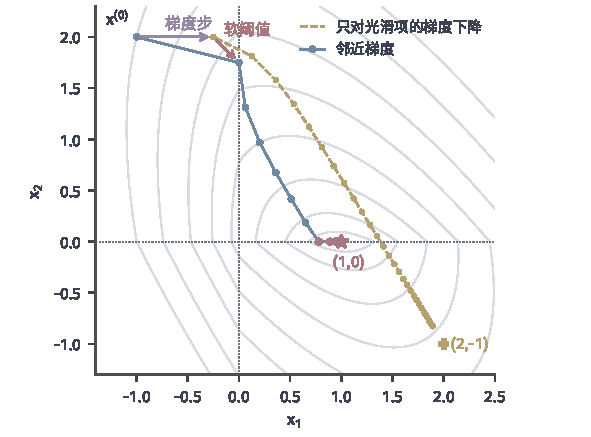
\includegraphics[width=100mm]{figures/03-optimization-evolution-and-signals/01-optimization/matplotlib/c4-lasso-path/figure.pdf}
  \caption{邻近梯度法在二维Lasso上的路径。灰色曲线是$F(\bm x)=\frac12\lVert\bm A\bm x-\bm b\rVert_2^2+\lVert\bm x\rVert_1$的等高线（$\bm A,\bm b$见例~\ref{ex:opt-ns-lasso-step}），红星是最小点$(1,0)$。蓝色折线是$\eta=1/4$的邻近梯度法，第一轮分解为紫色的梯度步和红色的软阈值；红色圆点标出第二个坐标恰为零的迭代点（从第7步起）。黄色虚线是只对光滑部分做梯度下降的路径，趋向光滑部分的最小点$(2,-1)$。}
  \label{fig:opt-ns-lasso-path}
\end{figure}

\paragraph{原目标的下降}
邻近梯度法近似了$f$，需要说明原目标$F$仍然受控。记$\bm x^+=\operatorname{prox}_{\eta r}(\bm x-\eta\nabla f(\bm x))$、$\bm d=\bm x^+-\bm x$。邻近最优条件（定理~\ref{thm:opt-ns-prox-characterization}的条件(2)）给出$-\bm d/\eta-\nabla f(\bm x)\in\partial r(\bm x^+)$；把这条次梯度的支撑不等式用于旧点$\bm x$，
\[
 r(\bm x)\geq r(\bm x^+)+\Bigl\langle-\frac{\bm d}\eta-\nabla f(\bm x),-\bm d\Bigr\rangle=r(\bm x^+)+\frac1\eta\lVert\bm d\rVert_2^2+\langle\nabla f(\bm x),\bm d\rangle .
\]
与下降引理$f(\bm x^+)\leq f(\bm x)+\langle\nabla f(\bm x),\bm d\rangle+\frac L2\lVert\bm d\rVert_2^2$相加，梯度项抵消，得
\begin{equation}
 F(\bm x^+)\leq F(\bm x)-\Bigl(\frac1\eta-\frac L2\Bigr)\lVert\bm x^+-\bm x\rVert_2^2 .
 \label{eq:opt-ns-proximal-gradient-descent}
\end{equation}
只要$0<\eta<2/L$，原目标就逐轮下降。这一推导没有用到$f$的凸性。

\paragraph{邻近梯度映射}
光滑优化用梯度范数衡量离驻点多远。复合目标的对应物是
\[
 \bm G_\eta(\bm x)=\frac{\bm x-\operatorname{prox}_{\eta r}\bigl(\bm x-\eta\nabla f(\bm x)\bigr)}\eta ,
\]
称为\term{邻近梯度映射}（proximal gradient mapping）。$r=0$时它就是$\nabla f(\bm x)$。它可以在每轮直接算出，并且有两条性质使它适合作停止量。

第一，$\bm G_\eta(\bm x)=\bm 0$当且仅当$\bm x$是邻近映射的不动点，由条件(2)这等价于$-\nabla f(\bm x)\in\partial r(\bm x)$，即$\bm 0\in\nabla f(\bm x)+\partial r(\bm x)$。称满足这一条件的点为复合目标的\term{复合临界点}（composite critical point），简称临界点。若$f$还是凸的，由于$f$在全空间有限，定理~\ref{thm:opt-ns-sum-rule}给出$\partial F=\nabla f+\partial r$，临界点就是全局最小点；$f$不凸时，它只是一阶必要条件。

第二，$\bm G_\eta(\bm x)$小，说明新点$\bm x^+$近似临界。由条件(2)，$\bm G_\eta(\bm x)-\nabla f(\bm x)\in\partial r(\bm x^+)$，所以向量$\nabla f(\bm x^+)-\nabla f(\bm x)+\bm G_\eta(\bm x)$属于$\nabla f(\bm x^+)+\partial r(\bm x^+)$，其范数不超过$L\lVert\bm x^+-\bm x\rVert_2+\lVert\bm G_\eta(\bm x)\rVert_2=(1+L\eta)\lVert\bm G_\eta(\bm x)\rVert_2$。

\paragraph{回溯与算法}
光滑常数$L$往往未知或偏保守。下降的证明只在一处用到$L$：新点满足二次上界。因此可以直接检验这个上界，不满足就缩小$\eta$重算。

\begin{algorithm}[带回溯的邻近梯度法]
  \label{alg:opt-ns-proximal-gradient}
  \begin{algorithmic}[1]
    \Require $f$的函数值与梯度，$r$的函数值与邻近映射；初值$\bm x^{(0)}\in\operatorname{dom}r$；初始步长$\eta>0$；缩小因子$\beta\in(0,1)$；容差$\varepsilon$
    \Ensure 近似临界点$\bm x$及其邻近梯度映射的范数
    \For{$t=0,1,2,\dots$}
      \State 计算$\nabla f(\bm x^{(t)})$
      \Loop
        \State $\bm x^+\gets\operatorname{prox}_{\eta r}\bigl(\bm x^{(t)}-\eta\nabla f(\bm x^{(t)})\bigr)$
        \If{$f(\bm x^+)\leq f(\bm x^{(t)})+\langle\nabla f(\bm x^{(t)}),\bm x^+-\bm x^{(t)}\rangle+\frac1{2\eta}\lVert\bm x^+-\bm x^{(t)}\rVert_2^2$}
          \State 跳出内层循环
        \EndIf
        \State $\eta\gets\beta\eta$
      \EndLoop
      \State $\bm x^{(t+1)}\gets\bm x^+$
      \If{$\lVert\bm x^{(t)}-\bm x^{(t+1)}\rVert_2/\eta\leq\varepsilon$}
        \State \Return $\bm x^{(t+1)}$
      \EndIf
    \EndFor
  \end{algorithmic}
\end{algorithm}

在算法~\ref{alg:opt-ns-proximal-gradient}中，检验条件一旦满足，上面的下降推导就可以把$L/2$换成$1/(2\eta)$，得到$F(\bm x^{(t+1)})\leq F(\bm x^{(t)})-\frac1{2\eta}\lVert\bm x^{(t+1)}-\bm x^{(t)}\rVert_2^2$。由下降引理，$\eta\leq1/L$时检验必然通过，所以步长不会缩小到$\beta/L$以下，内层循环有限次结束。每轮代价是一次梯度、若干次函数值与邻近映射；每次缩小步长都要重新计算邻近映射，因为中心变了。

\paragraph{固定预条件}
若用第~\ref{chap:opt-smooth}章的固定正定矩阵$\bm P$对梯度预条件，中心变成$\bm x-\eta\bm P\nabla f(\bm x)$，邻近步中的距离也必须换成相应的加权距离：
\[
 \bm x^+=\argmin_{\bm y}\Bigl\{r(\bm y)+\frac1{2\eta}\bigl(\bm y-\bm x+\eta\bm P\nabla f(\bm x)\bigr)^\top\bm P^{-1}\bigl(\bm y-\bm x+\eta\bm P\nabla f(\bm x)\bigr)\Bigr\}.
\]
这正是把模型中的$\frac1{2\eta}\lVert\bm y-\bm x\rVert_2^2$换成$\frac1{2\eta}(\bm y-\bm x)^\top\bm P^{-1}(\bm y-\bm x)$后配方的结果，相应的上界条件也要用这个加权距离检验。对角$\bm P=\operatorname{diag}(p_j)$配合$\ell_1$正则时，子问题仍然逐坐标分离，第$j$个坐标的阈值变为$\eta p_j\lambda$；一般的非对角$\bm P$会使子问题失去逐坐标的闭式解。只换中心而不换距离，所得更新的不动点一般不是原问题的临界点。

\paragraph{收敛保证}
下面在固定步长$0<\eta\leq1/L$下，分别对一般光滑项和凸光滑项给出保证。

\begin{theorem}[邻近梯度法的保证]
\label{thm:opt-ns-proximal-gradient}
设$F=f+r$如式~\eqref{eq:opt-ns-composite}，$0<\eta\leq1/L$固定，迭代~\eqref{eq:opt-ns-proximal-gradient}精确执行。
\begin{enumerate}
  \item 若$F$有下界$F_{\inf}>-\infty$，则$\displaystyle\min_{0\leq t<T}\lVert\bm G_\eta(\bm x^{(t)})\rVert_2^2\leq\frac{2\bigl(F(\bm x^{(0)})-F_{\inf}\bigr)}{\eta T}$。
  \item 若$f$还是凸的且最小点$\bm x^\star$存在，则$\displaystyle F(\bm x^{(T)})-F^\star\leq\frac{\lVert\bm x^{(0)}-\bm x^\star\rVert_2^2}{2\eta T}$。
\end{enumerate}
\end{theorem}

\begin{proof}
(1) $\eta\leq1/L$时$\frac1\eta-\frac L2\geq\frac1{2\eta}$，式~\eqref{eq:opt-ns-proximal-gradient-descent}化为$F(\bm x^{(t+1)})\leq F(\bm x^{(t)})-\frac\eta2\lVert\bm G_\eta(\bm x^{(t)})\rVert_2^2$。对$t=0,\dots,T-1$求和，左右相消后得$\frac\eta2\sum_t\lVert\bm G_\eta(\bm x^{(t)})\rVert_2^2\leq F(\bm x^{(0)})-F_{\inf}$，最小项不超过平均值。

(2) 先证一个三点不等式：对任意$\bm y$，记$\bm x^+$为$\bm x$的一步更新，
\begin{equation}
 F(\bm x^+)\leq F(\bm y)+\frac1{2\eta}\Bigl(\lVert\bm x-\bm y\rVert_2^2-\lVert\bm x^+-\bm y\rVert_2^2\Bigr).
 \label{eq:opt-ns-three-point}
\end{equation}
由下降引理与$\eta\leq1/L$，$f(\bm x^+)\leq f(\bm x)+\langle\nabla f(\bm x),\bm x^+-\bm x\rangle+\frac1{2\eta}\lVert\bm x^+-\bm x\rVert_2^2$；由$f$凸，$f(\bm x)\leq f(\bm y)-\langle\nabla f(\bm x),\bm y-\bm x\rangle$；由条件(2)给出的次梯度$\frac1\eta(\bm x-\bm x^+)-\nabla f(\bm x)\in\partial r(\bm x^+)$，$r(\bm x^+)\leq r(\bm y)+\langle\frac1\eta(\bm x-\bm x^+)-\nabla f(\bm x),\bm x^+-\bm y\rangle$。三式相加，含$\nabla f(\bm x)$的项全部抵消，得
\[
 F(\bm x^+)\leq F(\bm y)+\frac1\eta\langle\bm x-\bm x^+,\bm x^+-\bm y\rangle+\frac1{2\eta}\lVert\bm x^+-\bm x\rVert_2^2 .
\]
再用恒等式$2\langle\bm x-\bm x^+,\bm x^+-\bm y\rangle=\lVert\bm x-\bm y\rVert_2^2-\lVert\bm x^+-\bm y\rVert_2^2-\lVert\bm x-\bm x^+\rVert_2^2$，即得式~\eqref{eq:opt-ns-three-point}。取$\bm y=\bm x^\star$、$\bm x=\bm x^{(t)}$，对$t=0,\dots,T-1$求和，右端相消；由(1)中的单调性，$F(\bm x^{(T)})$不超过各轮目标值的平均，得结论。
\end{proof}

两条结论分别报告不同的对象。没有凸性时，只能保证某一轮的邻近梯度映射小，也就是找到一个近似临界点；这里的$O(1/T)$是平方残差的速率，残差本身是$O(1/\sqrt T)$，并且不说明临界点是否全局最优。$f$凸时，最后一个迭代点的目标差是$O(1/T)$，与第~\ref{chap:opt-smooth}章梯度下降在凸光滑目标上的速率相同：非光滑项$r$没有拖慢速率，代价是每轮多一次邻近映射。还要注意，每轮子问题的解$\bm x^{(t+1)}$只是当前模型的最小点，它与原问题最小点之间的差距，正是上面两条结论要控制的量，不能把“子问题已精确求解”误读为“原问题已解好”。

\subsection{加速邻近梯度法}
\label{sec:opt-ns-fista}

第~\ref{chap:opt-smooth}章的Nesterov加速梯度法在凸光滑目标上把$O(1/T)$提高到$O(1/T^2)$。它的做法是先沿上一步的位移外推，再在外推点求梯度。邻近梯度法可以用同样的方式加速，只需把梯度步换成邻近梯度步。

\paragraph{外推点与更新}
加速版本维护两个序列：记录点$\bm x^{(t)}$，以及只用于求梯度的外推点$\bm y^{(t)}$。每一轮在外推点上做一次邻近梯度步，得到新的记录点，再用新旧记录点的差外推出下一个求值点。外推系数由一个固定的数列确定。

\begin{algorithm}[加速邻近梯度法（FISTA）]
  \label{alg:opt-ns-fista}
  \begin{algorithmic}[1]
    \Require $f$的梯度，$r$的邻近映射；初值$\bm x^{(0)}$；步长$0<\eta\leq1/L$；迭代次数$T$
    \Ensure 记录点$\bm x^{(T)}$
    \State $\bm y^{(0)}\gets\bm x^{(0)}$，$\theta_0\gets1$
    \For{$t=0,1,\dots,T-1$}
      \State $\bm x^{(t+1)}\gets\operatorname{prox}_{\eta r}\bigl(\bm y^{(t)}-\eta\nabla f(\bm y^{(t)})\bigr)$ \Comment{在外推点求梯度}
      \State $\theta_{t+1}\gets\bigl(1+\sqrt{1+4\theta_t^2}\bigr)/2$
      \State $\beta^{(t)}\gets(\theta_t-1)/\theta_{t+1}$
      \State $\bm y^{(t+1)}\gets\bm x^{(t+1)}+\beta^{(t)}\bigl(\bm x^{(t+1)}-\bm x^{(t)}\bigr)$ \Comment{沿位移外推}
    \EndFor
  \end{algorithmic}
\end{algorithm}

算法~\ref{alg:opt-ns-fista}称为\term{加速邻近梯度法}（accelerated proximal gradient method），常用名FISTA\sidecite{beck2009fista}。它每轮的代价与邻近梯度法相同：一次梯度、一次邻近映射，外加两个向量的线性组合。系数$\beta^{(0)}=0$，此后依次约为$0.28,\ 0.43,\ 0.53,\dots$，逐渐趋于$1$。在例~\ref{ex:opt-ns-lasso-step}中，第一轮两种方法完全相同；从第二轮起外推开始起作用，前五轮的目标值分别为$4.03,\ 3.32,\ 2.67,\ 2.06,\ 1.56$，而邻近梯度法为$4.03,\ 3.32,\ 2.80,\ 2.38,\ 2.04$；到第10轮，两者的第一个坐标分别约为$0.997$和$0.972$（最优值为$1$）。

\begin{theorem}[加速邻近梯度法的目标差]
\label{thm:opt-ns-fista}
设$F=f+r$如式~\eqref{eq:opt-ns-composite}，$f$凸，最小点$\bm x^\star$存在，$0<\eta\leq1/L$，邻近映射精确计算。则算法~\ref{alg:opt-ns-fista}的记录点满足
\[
 F(\bm x^{(T)})-F^\star\leq\frac{2\lVert\bm x^{(0)}-\bm x^\star\rVert_2^2}{\eta(T+1)^2}.
\]
\end{theorem}

证明沿用第~\ref{chap:opt-smooth}章加速梯度法的势函数论证：把三点不等式~\eqref{eq:opt-ns-three-point}分别用于$\bm y=\bm x^{(t)}$和$\bm y=\bm x^\star$，按$\theta_t$加权组合，验证一个由目标差与到最小点距离组成的势函数逐轮不增；数列满足$\theta_{t+1}^2-\theta_{t+1}=\theta_t^2$及$\theta_t\geq(t+2)/2$，由此得到$(T+1)^2$的分母。完整推导见\sidecite[第4节]{beck2009fista}。与邻近梯度法相比，三点不等式是唯一用到$r$的地方；只要邻近步精确，非光滑项不影响加速论证。

\paragraph{加速不承诺单调}
定理只控制目标差的上界，不保证$F(\bm x^{(t)})$逐轮下降。外推点可能越过最小点，下一轮记录点的目标值随之上升。图~\ref{fig:opt-ns-ista-fista}在一个固定随机种子生成的Lasso问题上比较两种方法：$\bm A\in\mathbb R^{60\times100}$，奇数列与相邻偶数列高度相关，$\lambda$取$0.1\lVert\bm A^\top\bm b\rVert_\infty$，两种方法都用$\eta=1/L$。左图中，加速版本在第100轮的目标差约为$5\times10^{-6}$，而邻近梯度法约为$0.2$；右图放大后可见，加速版本的目标差呈波浪形起伏，600轮中有254轮目标值比上一轮更高。两条点线是定理~\ref{thm:opt-ns-proximal-gradient}与定理~\ref{thm:opt-ns-fista}给出的界，实际误差远在界以下：这些界是对所有满足条件的问题成立的最坏情形保证，而这个实例的局部曲率帮助两种方法都比界下降得快。

\begin{figure}[!htbp]
  \centering
  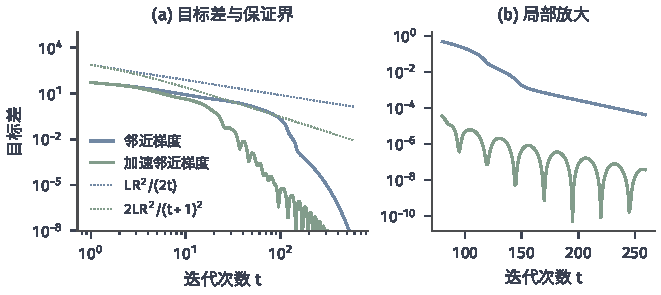
\includegraphics[width=112mm]{figures/03-optimization-evolution-and-signals/01-optimization/matplotlib/c4-ista-fista/figure.pdf}
  \caption{邻近梯度法与加速邻近梯度法在一个Lasso实例上的目标差（$n=60$，$d=100$，固定随机种子，参数见图源记录；$F^\star$由30000轮加速迭代估计）。(a) 双对数坐标下的$F(\bm x^{(t)})-F^\star$：蓝线为邻近梯度法，绿线为加速版本；点线为理论界$LR^2/(2t)$与$2LR^2/(t+1)^2$，$R=\lVert\bm x^{(0)}-\bm x^\star\rVert_2$。(b) 第80至260轮的放大（半对数坐标）：加速版本的目标差不单调，邻近梯度法单调下降。}
  \label{fig:opt-ns-ista-fista}
\end{figure}

\paragraph{实现时要配套的条件}
加速公式只是保证的一部分，以下几项改动都需要相应的条件。未知$L$时可以回溯，但检验必须在外推点$\bm y^{(t)}$处进行，即检验$f(\bm x^{(t+1)})\leq f(\bm y^{(t)})+\langle\nabla f(\bm y^{(t)}),\bm x^{(t+1)}-\bm y^{(t)}\rangle+\frac1{2\eta}\lVert\bm x^{(t+1)}-\bm y^{(t)}\rVert_2^2$，并且基本版本的分析要求步长只缩小、不放大。若需要单调的目标值，可以在目标上升时把外推系数重置为零，即“重启”；这在实践中常常有效，但重启后的速率需要另行分析，不能直接沿用定理~\ref{thm:opt-ns-fista}。邻近映射只能近似计算时，加速方法对误差更敏感：误差需要比非加速版本更快地趋于零，否则累积误差会抵消加速。$f$不凸时，上面的势函数论证不再成立，不能把$O(1/T^2)$的结论搬过去。
